\documentclass[conference]{IEEEtran}
\IEEEoverridecommandlockouts
% The preceding line is only needed to identify funding in the first footnote. If that is unneeded, please comment it out.
\usepackage{cite}
\usepackage{amsmath,amssymb,amsfonts}
\usepackage{algorithmic}
\usepackage{graphicx}
\usepackage{textcomp}
\usepackage{xcolor}
\usepackage{caption}
\usepackage{subcaption}
\usepackage{multirow}
\usepackage{url}
\def\BibTeX{{\rm B\kern-.05em{\sc i\kern-.025em b}\kern-.08em
    T\kern-.1667em\lower.7ex\hbox{E}\kern-.125emX}}
\begin{document}

\title{Image Processing and Computer Vision\\
}
\author{\IEEEauthorblockN{1\textsuperscript{st} George Lancaster}
\IEEEauthorblockA{\textit{dept. of Computer Science} \\
\textit{University of Bristol}\\
Bristol, United Kingdom \\
qv18258@bristol.ac.uk}
\and
\IEEEauthorblockN{2\textsuperscript{nd} Ren Jiang}
\IEEEauthorblockA{\textit{dept. of Computer Science} \\
\textit{University of Bristol}\\
Bristol, United Kingdom \\
mu18336@bristol.ac.uk}
}


\maketitle

\begin{abstract}
This report outlines the tasks completed for Image Processing and Computer Vision assignment one. Our final classifier, which uses template matching and speeded up robust features (SURF), has achieved an F1 score of 1 when tested against the sixteen test images. 
\end{abstract}

%%%%%%%%%%%%%%%%%%%%%%%%%%%%%%%%%%%
%%%%%%%%%%%%% Task 1 %%%%%%%%%%%%%%%%%%
%%%%%%%%%%%%%%%%%%%%%%%%%%%%%%%%%%%
\section{The Viola-Jones Object Detector}
\vspace{-0.15cm}
Sixteen test images were annotated for ground truth. Each test image contains either faces, dartboards or a combination of both. In this first task, the Viola-Jones object detector has been used to find faces within the test images \cite{viola2001rapid}. 
\begin{figure}[htb]
\centering
\begin{subfigure}{.5\linewidth}
  \centering
  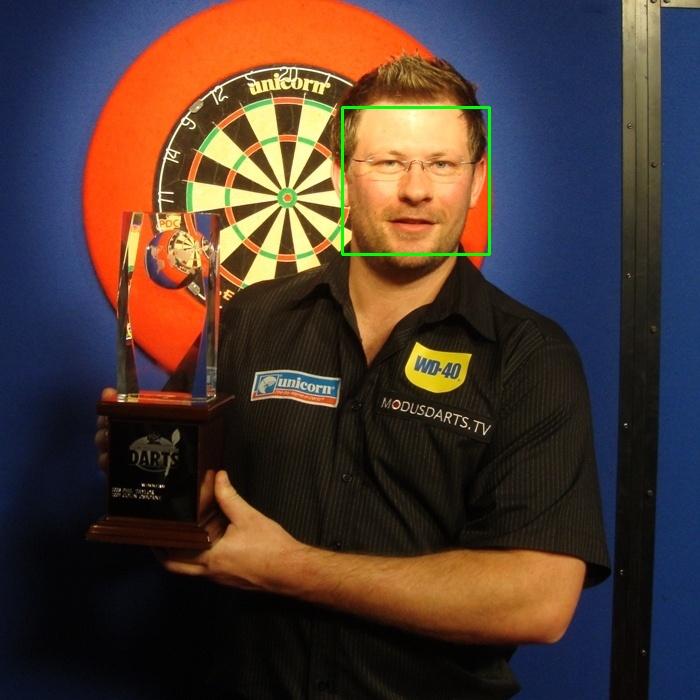
\includegraphics[width=.9\linewidth]{images/detected0.jpg}
  \caption{darts4}
  \label{fig:sub1}
\end{subfigure}%
\begin{subfigure}{.5\linewidth}
  \centering
  \vspace{0.6cm}
  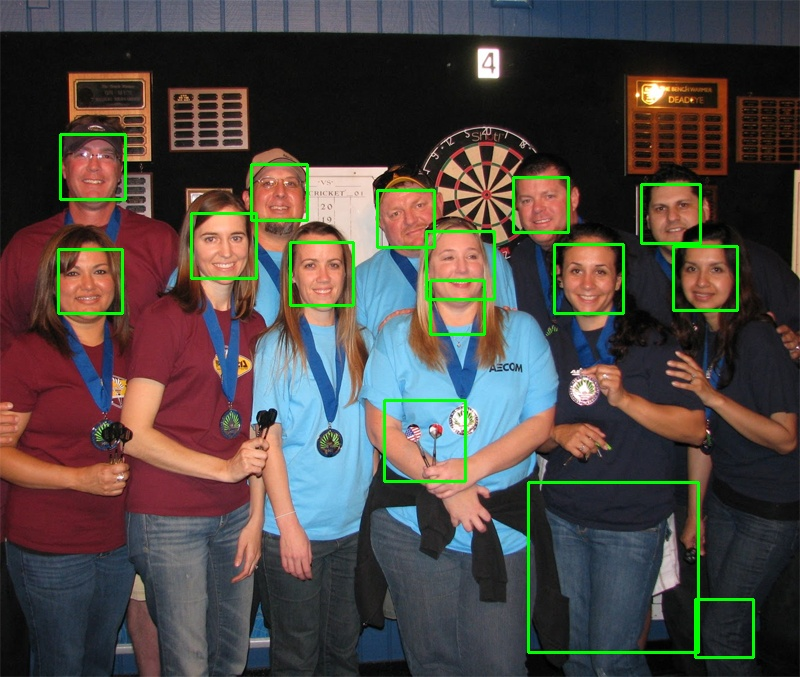
\includegraphics[width=.9\linewidth]{images/detected1.jpg}
  \caption{darts5}
  \label{fig:sub2}
\end{subfigure}
\begin{subfigure}{.5\linewidth}
  \centering
    \vspace{0.2cm}
  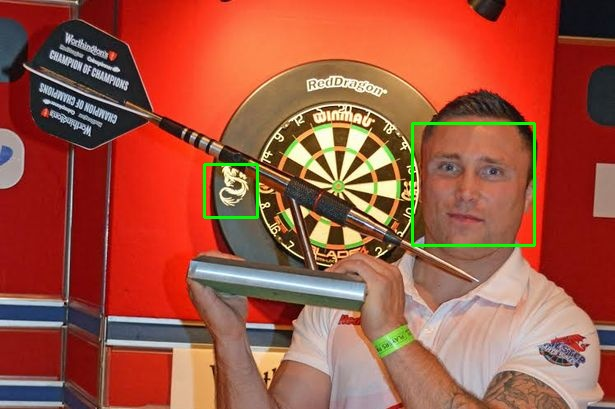
\includegraphics[width=.9\linewidth]{images/detected2.jpg}
  \caption{darts13}
  \label{fig:sub1}
\end{subfigure}%
\begin{subfigure}{.5\linewidth}
  \centering
      \vspace{0.7cm}
  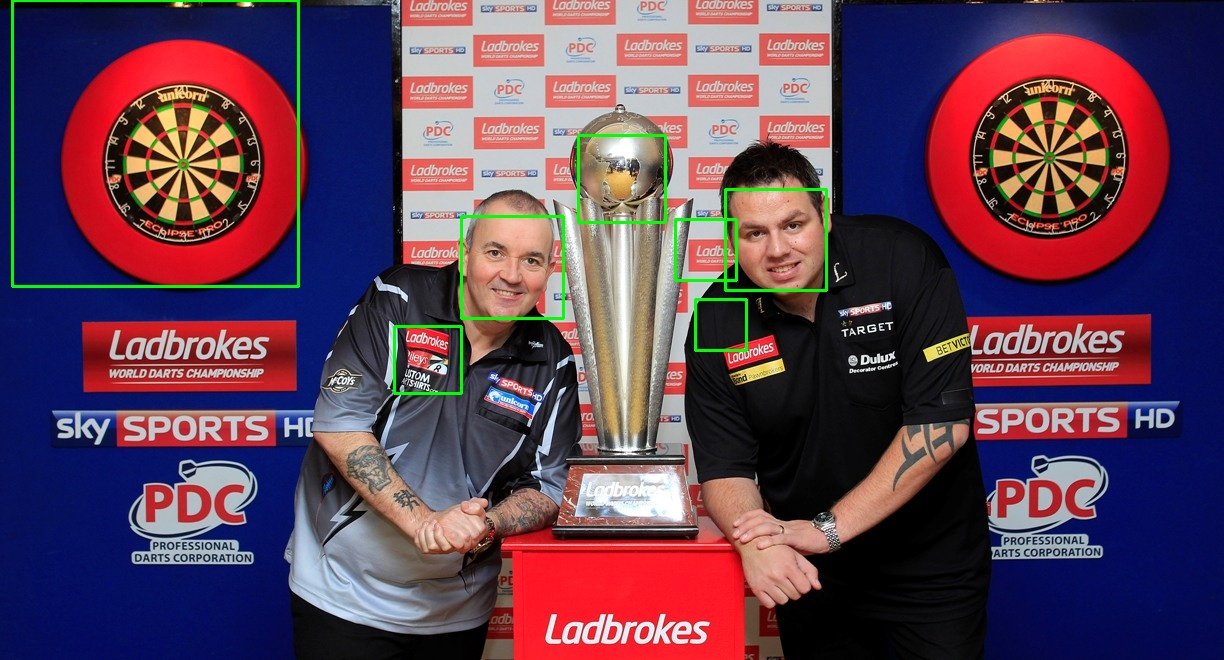
\includegraphics[width=.9\linewidth]{images/detected3.jpg}
  \caption{darts14}
  \label{fig:sub2}
\end{subfigure}
\begin{subfigure}{.5\linewidth}
\centering
    \vspace{0.2cm}
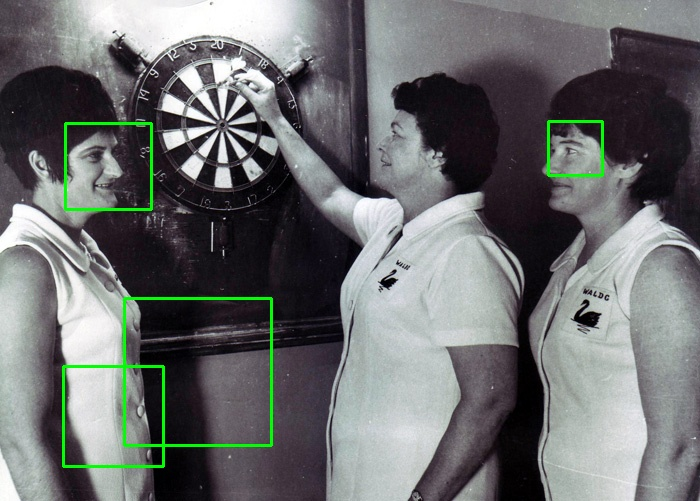
\includegraphics[width=0.9\linewidth]{images/detected4.jpg}
\caption{darts15}
\end{subfigure}


\caption{Five images from the test data set. Green rectangles show where the Viola-Jones classifier has detected a face. }
\label{fig:q13}
\end{figure}
\par 
The true positive rate for images \emph{darts5} and \emph{darts15} when tested using the Viola-Jones face detector are 1 and 0.67 respectively. 
\par
Although the true positive rate can be used to indicate a classifiers accuracy, it does not reflect its true performance. It is always possible to get a 100 per cent detection rate on any classification task as we can select all possible areas of an image, regardless of the number of false positives. The key to a good classifier is to get a high true positive rate, whilst keeping the false positive rate minimal. The F1 score measures the relationship between the precision and the recall of the model and can therefore be considered to be a more reliable measure of classifier performance.
\par
Additionally, the true positive rate can be difficult to assess as it requires the definition of a rule to determine what counts as a detection. For this task, a true detection is defined as an area that shares a 68 per cent overlap with a ground truth annotation. A value of 68 per cent was chosen as it is the largest area of overlap before the F1 score starts to decline. 
\par 
\begin{table}[htp]
\caption{F1 scores, precision and recall for all sixteen test images, when detecting faces using the Viola-Jones face detector.}
\begin{center}
\begin{tabular}{||c|c|c|c||}
\hline
Image Name			 	& F1 Score 	& Precision	& Recall            \\ \hline
dart0						& 1.00		&	1.00		& 1.00		\\
dart1						& 1.00		&	0.00		& 0.00		\\
dart2						& 1.00		&	0.00		& 0.00		\\
dart3						& 1.00		&	0.00		& 0.00		\\
dart4						& 1.00		&	1.00		& 1.0	0		\\
dart5						& 0.79		&	0.65		& 1.00		\\
dart6						& 1.00		&	0.00		& 0.00		\\
dart7						& 1.00		&	1.00		& 0.00		\\
dart8						& 1.00		&	0.00		& 0.00		\\
dart9						& 0.67		&	0.50		& 1.00		\\
dart10					& 1.00		&	0.00		& 0.00		\\
dart11					& 0.67		&	1.00		& 0.50		\\
dart12					& 1.00		&	0.00		& 0.00		\\
dart13					& 1.00		&	1.00		& 1.00		\\
dart14					& 0.36		&	0.22		& 1.00		\\
dart15					& 0.40		&	0.50		& 0.33		\\ \hline
Average F1 Score 		 	&	\multicolumn{3}{c||}{0.87} 			\\ \hline
\end{tabular}
\end{center}
\label{default}
\end{table}
\par
Using the Viola-Jones face detector gives fair results when applied to the 16 test images. Images that have been correctly classified as containing no faces have been given an F1 score of 1. When excluding these images from the calculation, the F1 score is reduced to 0.81.



%%%%%%%%%%%%%%%%%%%%%%%%%%%%%%%%%%%
%%%%%%%%%%%%% Task 2 %%%%%%%%%%%%%%%%%%
%%%%%%%%%%%%%%%%%%%%%%%%%%%%%%%%%%%

\newpage
\section{The Dartboard Detector}
To detect dartboards, the Viola-Jones classifier was trained on a data set generated from a single bitmap image of a dartboard, in addition to a set of negative images. 
\begin{figure}[htbp]
\begin{center}
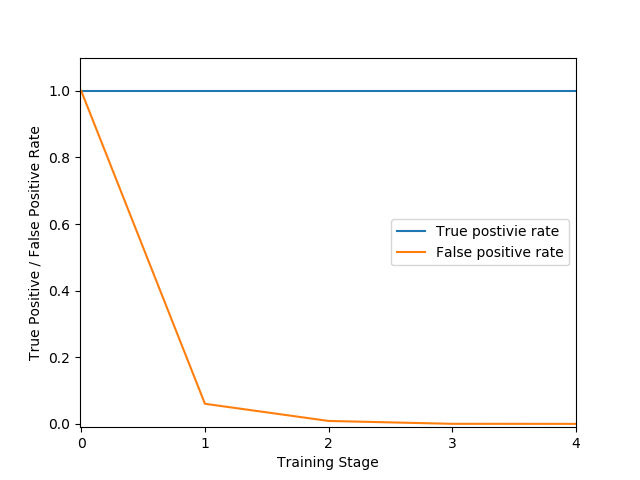
\includegraphics[width=1\linewidth]{images/TPRvsFPR}
\caption{True positive rate plotted against false positive rate when training the cascade classifier on 500 images of dartboards and 500 negative images over four stages (0-4). }
\label{default}
\end{center}
\end{figure}
\par

On the first stage of training, all samples are classified as true. This is reflected by a value of 1 for both the true positive rate and false positive rate. As the classifier progresses through further training stages, the false positive rate decreases, whilst the true positive rate remains the same. This indicates that the classifier improved after each training stage by decreasing the number of false detections only. 
\begin{table}[!htb]
\caption{F1 scores for all sixteen test images when detecting dartboards, using the Viola-Jones cascade classifier trained on dartboards.}
\begin{center}
\begin{tabular}{||c|c|c||}
\hline
\multirow{2}{*}{Image Name} & \multicolumn{2}{c||}{F1 Score}                \\ 
                                 & 500 Training Images	& 1000 Training images \\ \hline
dart0				& 0.5	0	&	0.25	\\
dart1				& 0.00	&	0.50	\\
dart2				& 0.25	&	0.40	\\
dart3				& 0.54	&	0.33	\\
dart				& 0.4	0	&	0.25	\\
dart5				& 0.15	&	0.20	\\
dart6				& 0.33	&	0.50	\\
dart7				& 0.00	&	0.25	\\
dart8				& 0.16	&	0.25	\\
dart9				& 0.22	&	0.20	\\
dart10			& 0.40	&	0.55	\\
dart11			& 0.22	&	0.22	\\
dart12			& 0.67	&	0.50	\\
dart13			& 0.20	&	0.33	\\
dart14			& 0.09	&	0.14	\\
dart15			& 0.67	&	0.50	\\ \hline
Average F1 score 	& 0.28	&	0.34	\\ \hline
\end{tabular}
\end{center}
\label{default}
\end{table}%
\newpage
\par
To measure how varying the number of training images affects performance, two identical Viola-Jones classifiers were trained on sets of 500, and 1000 true images and negatives. Training on 1000 images improved the F1 score by 0.06. This suggests that the classifiers performance can be improved by increasing the amount of training data. 

\par
Observed differences in accuracy between training and testing can be attributed to the training data consisting of a small set of critical features. In contrast, the test images contain a large amount of irrelevant background noise, which needs to be discarded by the cascade. Because of this, the false positive rate is much higher for the test images. 
\par
\begin{figure}[htb]
\centering
\begin{subfigure}{.5\linewidth}
  \centering
  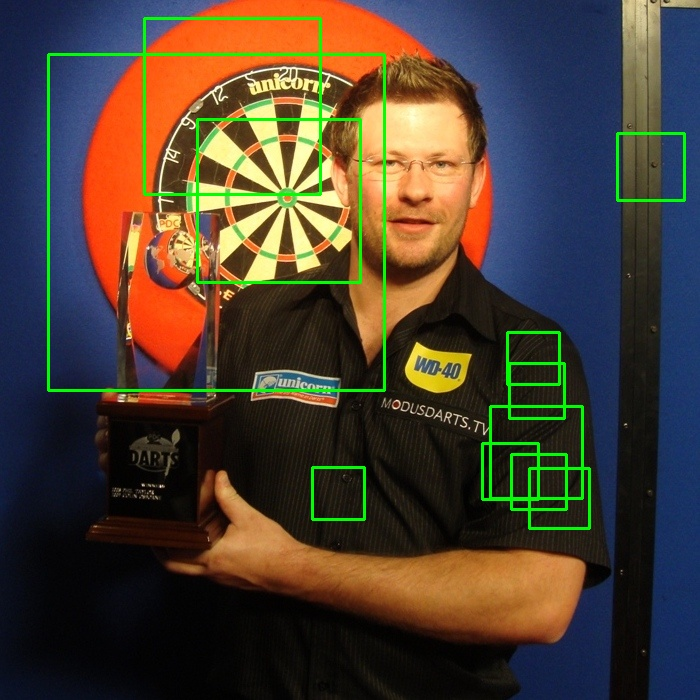
\includegraphics[width=.9\linewidth]{images/task2/detected4.jpg}
  \caption{darts4}
  \label{fig:sub1}
\end{subfigure}%
\begin{subfigure}{.5\linewidth}
  \centering
  \vspace{0.7cm}
  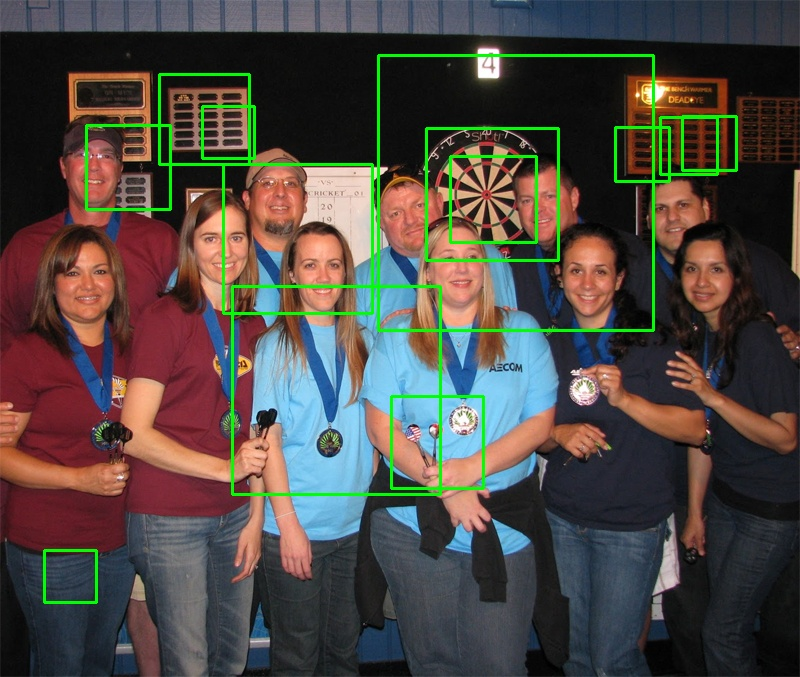
\includegraphics[width=.9\linewidth]{images/task2/detected5.jpg}
  \caption{darts5}
  \label{fig:sub2}
\end{subfigure}
\begin{subfigure}{.5\linewidth}
  \centering
    \vspace{0.2cm}
  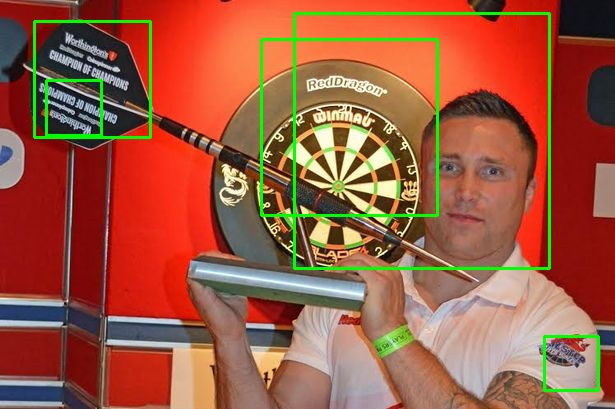
\includegraphics[width=.9\linewidth]{images/task2/detected13.jpg}
  \caption{darts13}
  \label{fig:sub1}
\end{subfigure}%
\begin{subfigure}{.5\linewidth}
  \centering
    \vspace{0.7cm}
  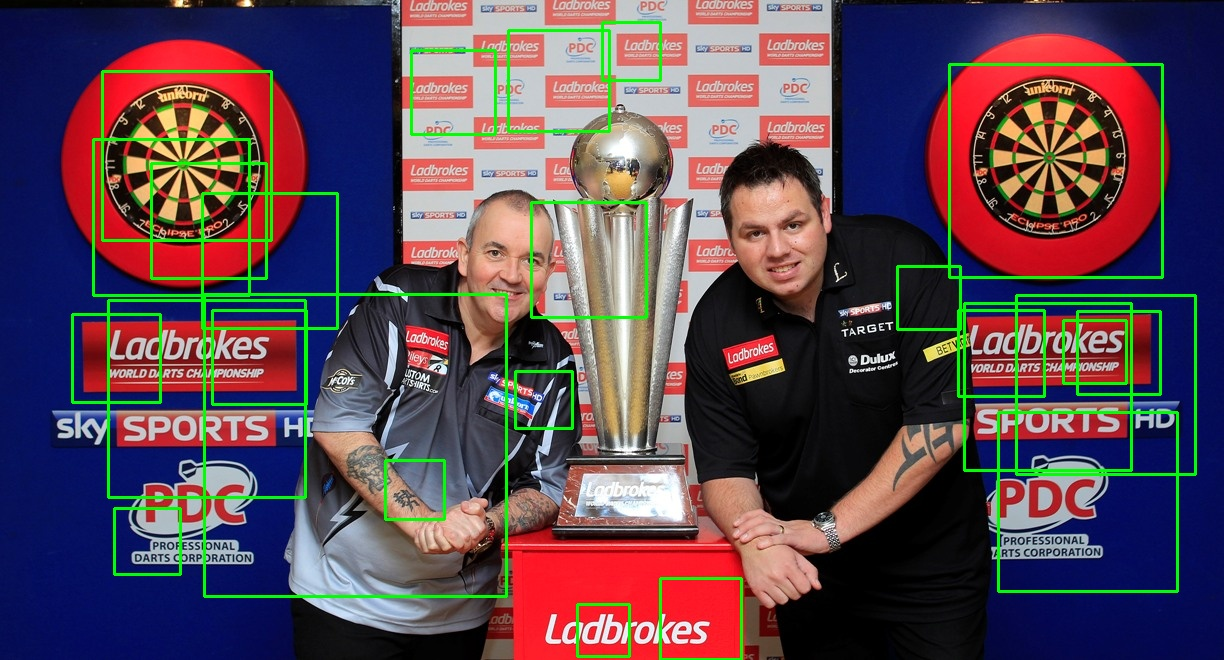
\includegraphics[width=.9\linewidth]{images/task2/detected14.jpg}
  \caption{darts14}
  \label{fig:sub2}
\end{subfigure}
\caption{Four images from the test data set. Green rectangles show where the Viola-Jones classifier has detected a dartboard.}
\end{figure}
\par
The performance of the dartboard detector at this stage is remarkably worse than the face detector from task one. One reason for this being that the face detection classifier has been trained on a larger number of stages, which means that there is more opportunity for false positives to be filtered out from the result. This is supported by a recall value of 1 for the dartboard classifier, meaning that all dartboards have been successfully detected. However, the precision of 0.21 brings the F1 score down. 
\par
Additionally, the face detector has been trained on a much larger data set than the dartboard detector. We propose that further increasing the size and variety of the training data could increase the precision of the model. 

%%%%%%%%%%%%%%%%%%%%%%%%%%%%%%%%%%%
%%%%%%%%%%%%% Task 3 %%%%%%%%%%%%%%%%%%
%%%%%%%%%%%%%%%%%%%%%%%%%%%%%%%%%%%
\clearpage
\section{Integration with Shape Detectors}
Both linear and circular hough transforms have been used in conjunction with the Viola-Jones classifier to improve the precision and recall of the system. 
\par
\begin{table}[htp]
\caption{F1 scores, precision and recall for all images, when detecting for dartboards using the Viola-Jones classifier combined with shape detection techniques. }
\begin{center}
\begin{tabular}{||c|c|c|c||}
\hline
Image Name		 	& F1 Score 	& Precision	& Recall            \\ \hline
dart0					& 1.00		&	1.00		& 1.00		\\
dart1					& 1.00		&	1.00		& 1.00		\\
dart2					& 1.00		&	1.00		& 1.00		\\
dart3					& 1.00		&	1.00		& 1.00		\\
dart4					& 1.00		&	1.00		& 1.00		\\
dart5					& 1.00		&	1.00		& 1.00		\\
dart6					& 1.00		&	1.00		& 1.00		\\
dart7					& 1.00		&	1.00		& 1.00		\\
dart8					& 1.00		&	1.00		& 1.00		\\
dart9					& 0.67		&	0.50		& 1.00		\\
dart10				& 1.00		&	1.00		& 1.00		\\
dart11				& 1.00		&	1.00		& 1.00		\\
dart12				& 1.00		&	1.00		& 1.00		\\
dart13				& 1.00		&	1.00		& 1.00		\\
dart14				& 0.67		&	0.50		& 1.00		\\
dart15				& 1.00		&	1.00		& 1.00		\\ \hline
Average 		 		& 0.96		&	0.94		& 1.00 		\\ \hline
\end{tabular}
\end{center}
\label{default}
\end{table}
\par
The solution at this level gives very good results, achieving a true positive rate of 1 for all images. Only images 9 and 14 have imperfect F1 scores, caused by false positives. Image 9 could be considered to be a true positive as the classifier has detected a dartboard on a t-shirt. 
\par

\begin{figure}[htbp]
\begin{center}
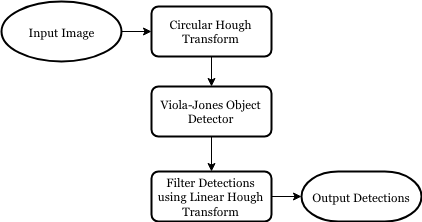
\includegraphics[width=1\linewidth]{images/flowdiagram.png}
\caption{Flow diagram of image detection algorithm. }
\label{default}
\end{center}
\end{figure}
\par
The circular hough transform has been used to detect areas of interest for the Viola-Jones classifier. For any group of intersecting detected circles, the centre of mass is found by plotting all detections on a blank image and using the OpenCV  function \emph{findContours} \cite{suzuki1985topological}. This algorithm scans the image, it is interrupted when an edge has been detected. In this case, an edge is any non-zero value. Through following the border of the first detected edge, an outline of a shape can be mapped and added to a list of detected features.
\par 
Reasons  for building the classifier in this way include: 
\begin{itemize}
\item Although the Viola-Jones classifier can filter out background information, applying the hough transform first allows it to focus on areas of interest; 
\item Each area is checked by the linear hough transform to ensure that there is a dartboard present. Twenty-five intersecting lines indicates truth. 
\end{itemize}

\begin{figure}[htb]
\centering
\begin{subfigure}{.5\linewidth}
  \centering
  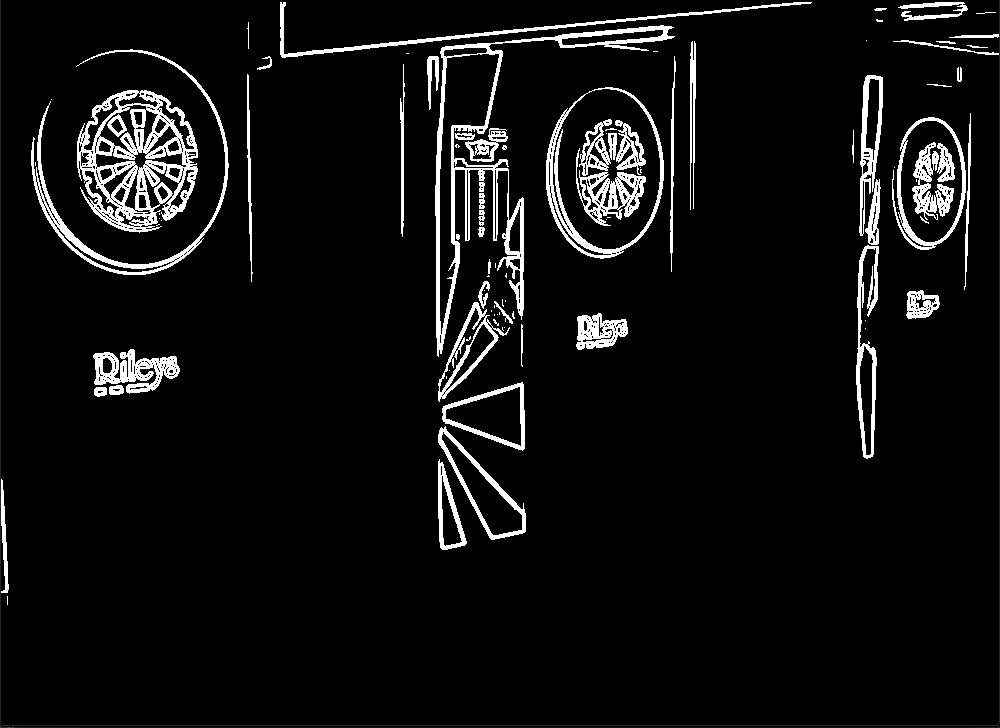
\includegraphics[width=.9\linewidth]{images/task3/bestthresh.png}
  \caption*{Gradient threshold}
  \label{fig:sub1}
\end{subfigure}%
\begin{subfigure}{.5\linewidth}
\vspace{0.78cm}
  \centering
  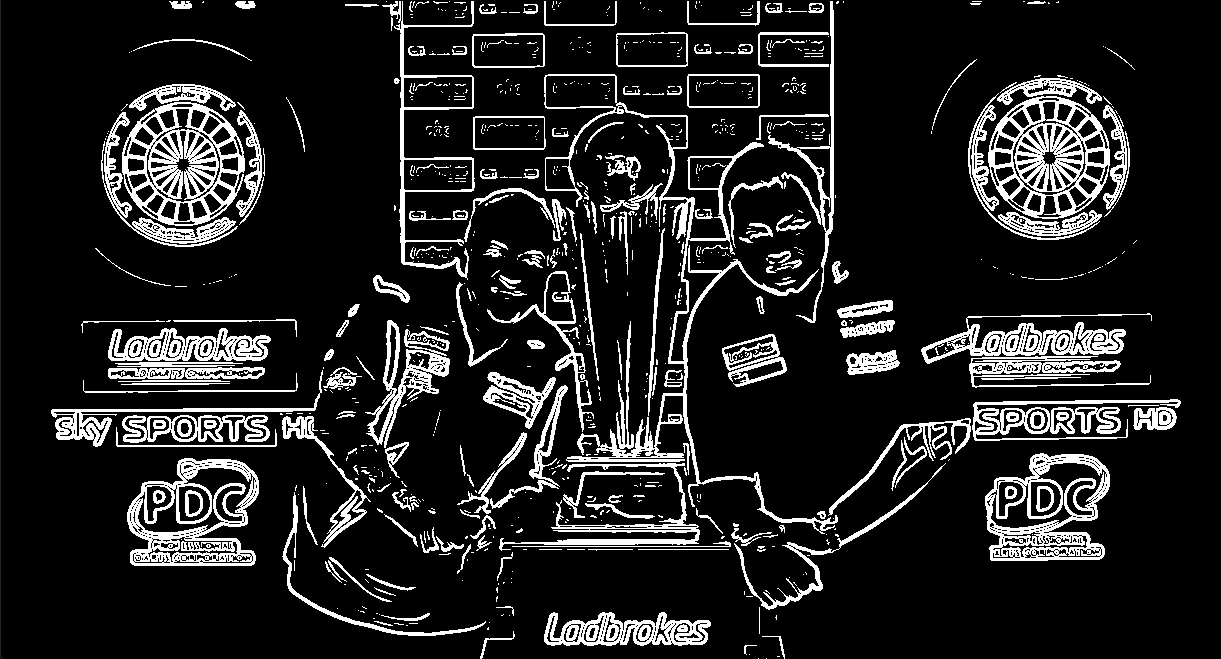
\includegraphics[width=.9\linewidth]{images/task3/worstthresh.png}
  \caption*{Gradient threshold}
  \label{fig:sub2}
\end{subfigure}
\begin{subfigure}{.5\linewidth}
\vspace{0.3cm}
  \centering
  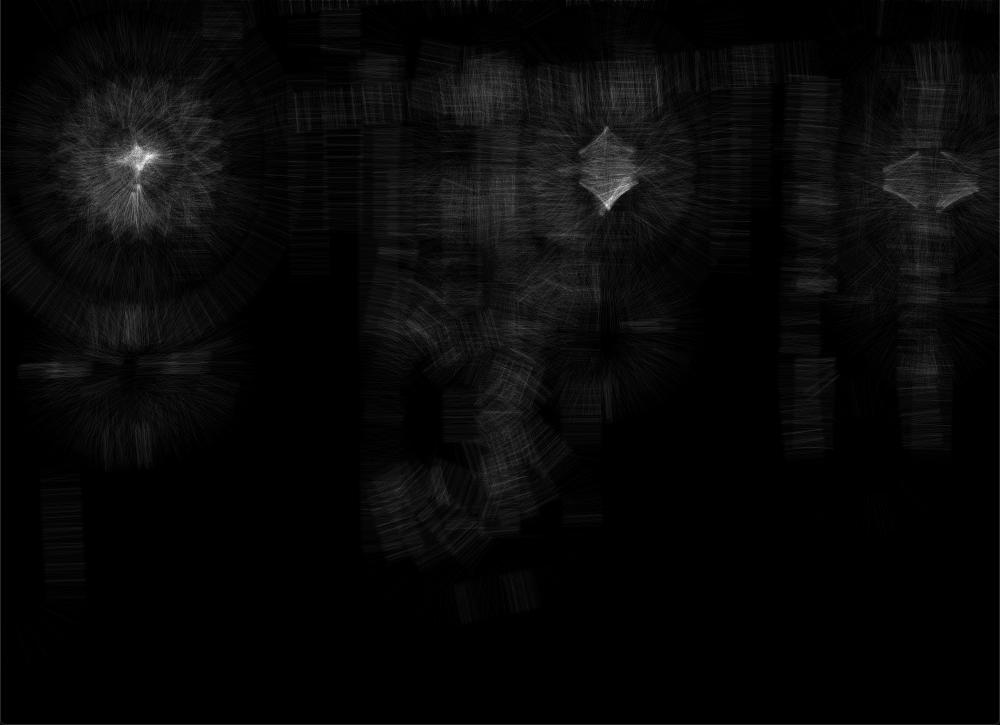
\includegraphics[width=.9\linewidth]{images/task3/bestcirclehough.png}
  \caption*{Circular Hough Transform}
  \label{fig:sub1}
\end{subfigure}%
\begin{subfigure}{.5\linewidth}
\vspace{1.1cm}
  \centering
  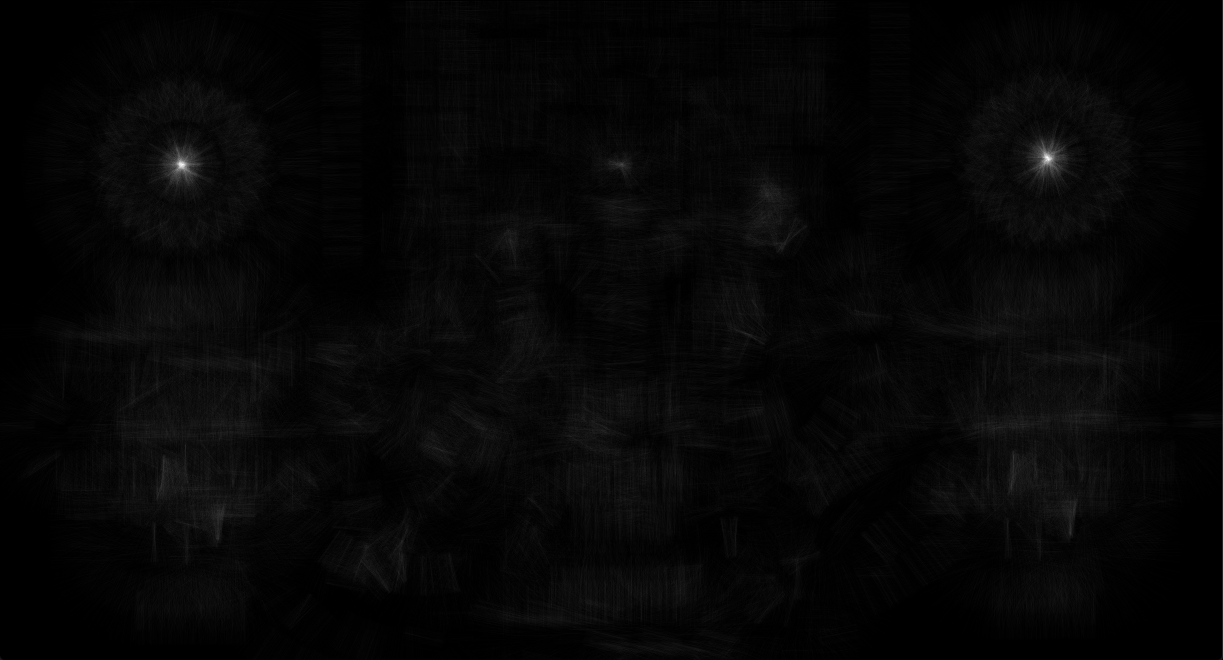
\includegraphics[width=.9\linewidth]{images/task3/worstcirclehough.png}
  \caption*{Circular Hough Transform}
  \label{fig:sub2}
\end{subfigure}

\begin{subfigure}{.5\linewidth}
\vspace{0.3cm}
  \centering
  \captionsetup{justification=centering}
  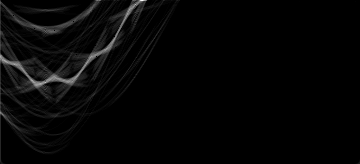
\includegraphics[width=.9\linewidth]{images/task3/houghlinebest.png}
  \caption*{Hough Line Transform \\for a Single Dartboard}
  \label{fig:sub1}
\end{subfigure}%
\begin{subfigure}{.5\linewidth}
\captionsetup{justification=centering}
\vspace{0.3cm}
  \centering
  
\includegraphics[width=.9\linewidth]{images/task3/houghlineworst.png}
  \caption*{Hough Line Transform \\for a Single Dartboard}
  \label{fig:sub2}
\end{subfigure}



\begin{subfigure}{.5\linewidth}
\vspace{0.3cm}
  \centering
  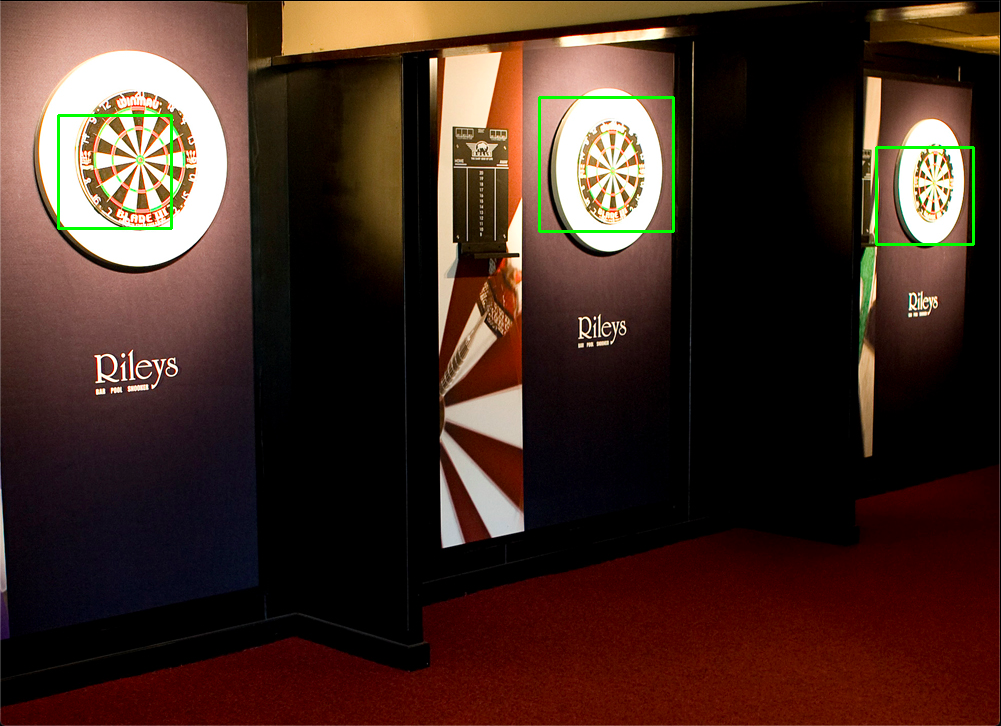
\includegraphics[width=.9\linewidth]{images/task3/bestresult.png}
  \caption{Detected Area}
  \label{fig:sub1}
\end{subfigure}%
\begin{subfigure}{.5\linewidth}
\vspace{1.1cm}
  \centering
  
\includegraphics[width=.9\linewidth]{images/task3/worstresult.png}
  \caption{Detected Area}
  \label{fig:sub2}
\end{subfigure}
\caption{Best and worst cases for the dartboard detector. Column a shows the best case \emph{dart8}, which has a F1 score of 1.  Column b shows the worst case \emph{dart14}, which has an F1 score of 0.67}
\end{figure}


Merits of the classifier include: 
\begin{itemize}
	\item It has a perfect recall value for all images;
	\item The false positive rate is very low, with only three false positives in the entire data set.
\end{itemize}
And the shortcomings include:
\begin{itemize}
	\item The classifiers parameters have been tuned to perform well on the test data set, it may not generalise well to other images;
	\item Classification speed is slow due to the hough transform. It could not be applied to data in real-time. 
\end{itemize}




%%%%%%%%%%%%%%%%%%%%%%%%%%%%%%%%%%%
%%%%%%%%%%%%% Task 4 %%%%%%%%%%%%%%%%%%
%%%%%%%%%%%%%%%%%%%%%%%%%%%%%%%%%%%
\newpage
\section{Further Improvements}
As the dartboard detector from part three has perfect precision, improvement can only be made to the recall. Two filters, using SURF and template matching have been used as final layers in the dartboard detector to reduce the number of false positives, and achieve a perfect F1 score for the test data set. 
\par
\subsection{Speeded up robust features (SURF)}
SURF aims to map the relationship between a descriptor and detector to find similarities in images \cite{bay2006surf}. The SURF algorithm splits object detection into three stages: interest point detection, local neighbourhood description and matching. Interest point detection performs blob detection to detect characteristic regions in the object image. Local neighbourhood description uses the points of interest to define the features of the image. By comparing descriptors from two images, matching pairs of points of interest can be found \cite{surf_site}. 
\par

\begin{figure}[!htb]
\begin{center}
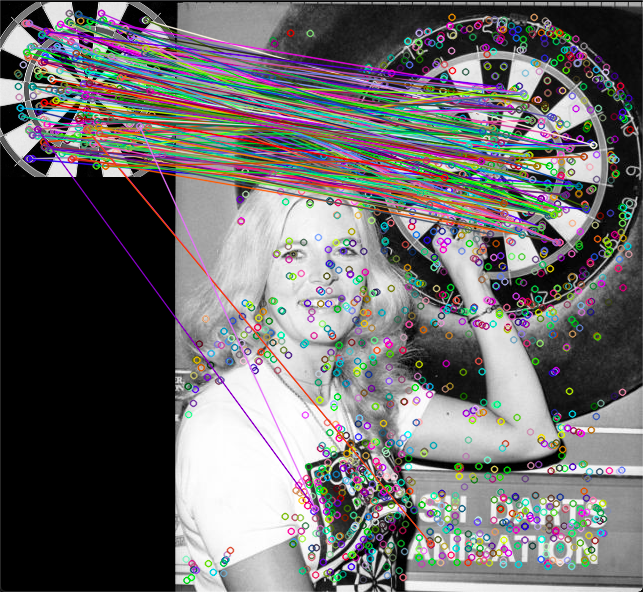
\includegraphics[width=0.6\linewidth]{images/SURF.png}
\caption{SURF, applied to \emph{dart9}. Because there are not enough points of interest on the t-shirt, the feature is excluded from the number of detections. }
\label{default}
\end{center}
\end{figure}
\par
By applying SURF as a filter, only areas with more than two significant points of interest have been kept in the list of detected dartboards.



\subsection{Template Matching}
Template matching is used to  match parts of an image to a template. The dartboard used from part two only has 3 layers, therefore it lacks the later layers that remove falsely detected features. By having more layers, the false positive rate can be reduced \cite{lewis1995fast}. \par

Through experimentation, a template has been found that rejects false positives, whilst keeping the true positives.  
\par 
\begin{figure}[!htb]
\begin{center}
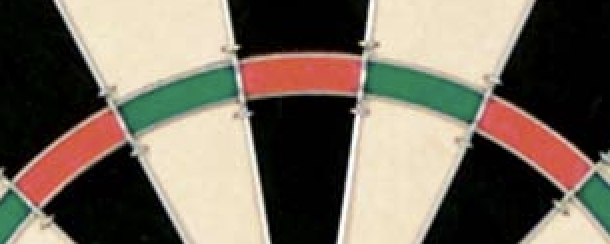
\includegraphics[width=0.8\linewidth]{images/template.png}
\caption{The template used in the template matching extension. }
\label{default}
\end{center}
\end{figure}

\par 
\begin{figure}[!htb]
\begin{center}

\includegraphics[width=0.8\linewidth]{images/template_merit.jpg}
\caption{Template matching rejects the two remaining false positives from \emph{dart15}.}
\label{default}
\end{center}
\end{figure}
The key to successful template matching is to choose a template with enough features to reject false areas. However, it shouldn't contain all the features of a dartboard because there may be shelters, irregular shapes or light in the test images that prevent them from getting high enough scores. Therefore, many different templates should be tried before a suitable one can be used.

\subsection{Results}
Applying the SURF filter removes two false positives. One from dart9, and one from dart14. This leaves one false positive in dart14, which is removed by template matching. 
\par
We have decided to exclude a dartboard from \emph{dart8} and \emph{dart11} due to too much noise in the image. 
\begin{table}[!htp]
\caption{F1 scores, precision and recall for all images, when detecting for dartboards using the Viola-Jones classier combined with shape detection techniques, SURF and template matching. }
\begin{center}
\begin{tabular}{||c|c|c|c||}
\hline
Classifier task		 	& F1 Score 	& Precision	& Recall            \\ \hline
task 2				& 0.28		&	0.29		& 1.00		\\
task 3				& 0.96		&	0.94		& 1.00		\\
task 4				& 1.00		&	1.00		& 1.00		\\\hline

\end{tabular}
\end{center}
\label{default}
\end{table}
\bibliography{citations}
\bibliographystyle{unsrt}


\end{document}